\chapter{Estado del arte}
En este capítulo se exponen los principales temas de interés para la realización de este trabajo, las investigaciones realizadas sobre la TPV y NF-TPV (termofotovoltaica de campo cercano) y el marco teórico sobre las diferentes maneras que se transmite el calor.

\section{Termo-fotovoltaica}
Un generador termo-fotovoltaico(TPV) se basa en la conversión de energía calorífica en energía eléctrica mediante el efecto fotovoltaico a través una célula termo-fotovoltaica sin requerir ninguna parte móvil, conocido este tipo de sistemas de generación como motores pasivos de calor, como se representa de una manera sencilla en la figura \ref{fig:TPV_Subsistema}. El emisor se encuentra a una alta temperatura lo cual produce que se transmite el calor en forma de radiación que al llegar a la célula es reflejada, transmitida o absorbida, la porción de radiación absorbida excita a los electrones produciendo un par electrón-hueco sí solo sí la energía del fotón absorbido es mayor que la energía de la banda energética de la célula, al conectar los terminales de la célula a una carga se produce una corriente que alimenta a la carga proporcional a la intensidad lumínica, aquellos fotones con energía menor a la banda energética son suprimidos o reflejados para disminuir el flujo de calor\cite{Present_Efficiencies_and_Future_Opportunities_in_Thermophotovoltaics}.\\

\begin{figure}[H]
	\centering
	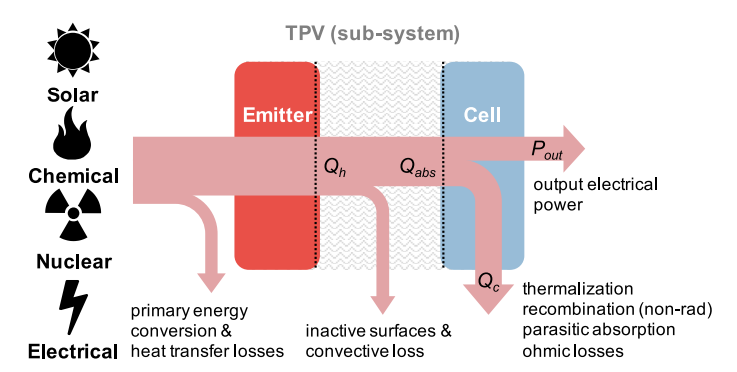
\includegraphics[width=0.7\textwidth]{figuras/TPV_Subsistema.png}
	\caption{Flujo de conversión de la energía térmica en energía eléctrica. \textit{Fuente: \cite{Present_Efficiencies_and_Future_Opportunities_in_Thermophotovoltaics}}}
	\label{fig:TPV_Subsistema}
\end{figure}

La termofotovoltaica ha sido un campo de interés para aplicaciones militares, espaciales, generación de electricidad y recuperación de calor residual. Para la milicia de los Estados Unidos de América se han conducido varias investigaciones para la búsqueda de un generador silencioso y portátil \cite{military_TPV}, cumpliéndose en 2004 40 años de investigación sin conseguirse potencias por encima de 500W \cite{military_TPV_40Years}. En aplicaciones espaciales es de interés por presentar beneficios en rendimiento para misiones cercanas al Sol y misiones en el espacio profundo porque los componentes más sensibles se encuentran resguardados de la dura radiación, siendo posible también el guardar energía en gravedad cero \cite{TPV_space_applications}. Para la recuperación de calor residual existe un gran interés porque la conversión de energía térmica a eléctrica es menor del 40\% en las plantas de generación de energía de combustibles fósiles convencionales, produciéndose una gran cantidad de pérdidas en forma de calor \cite{wasteHeat_TPV}.\\

Todas estas áreas de interés ha provocado un aumento de las investigaciones en los sistemas de generación termo-fotovoltaicos, estudiándose la utilización de células multibandas \cite{MultiEstados_Capas_TPVs}, diferentes materiales de emisor para aumentar la potencia radiada, aplicación de capas finas en el emisor para el aumento de la potencia radiada\cite{doi:Near_field_ThinFilm}, aplicación de filtros \cite{multiLayerFilters} y capas reflectantes para la recuperación de fotones y disminución de calentamiento\cite{Thermoionic_nTPV_DATAS201910},la combinación con un TEC para aumentar la densidad de potencia y eficiencia total del sistema generador\cite{thermoionic_TPV_NF,progress_Thermoionic_TPV,Thermoionic_nTPV_DATAS201910}, y la disminución del espacio entre emisor y célula para aprovechar los efectos de la radiación de campo cercano\cite{thermoionic_TPV_NF,modelEfficiency_NF_TPV,nf_TPV_Pillars_SiO2}.\\
%\cite{thermoionic_TPV_NF,modelEfficiency_NF_TPV,nf_TPV_Pillars_SiO2,NearField_200nm}

Las investigaciones no se han limitado a estudiar células TPV de una o varias uniones p-n, sino también la utilización de células termofotovoltaicas interbandas en cascada(ICTPV) de banda energéticas comprendidas entre 0.2 y 0.5 eV que resulta en una eficiente colección de portadores foto-generados, donde la eficiencia máxima($\eta_max$) y la diferencia de potencial en vacío($V_{OC}$) es proporcional a el número de bandas (stages) hasta unos 0.691 V de $V_{OC}$ y uno 6.2\% $\eta_{max}s$, pero genera una significante cantidad de energía térmica por la densidad de corriente oscura\cite{MultiEstados_Capas_TPVs}. Esta corriente se consigue disminuir al introducir una barrera entre las capas \cite{decreaseDarkCurrent}.\\

Aunque todavía quedan por estudiar muchos materiales y disposiciones del emisor y de la célula, algo de alta importancia es el estudio de filtros y capas reflectantes porque permiten la re-utilización de los fotones no absorbidos, aumentando la eficiencia y evitando que se acabe calentando innecesariamente la célula. Las capas traseras reflectantes(BSR), principalmente hechas de oro, reducen las pérdidas de radiación que es la absorción de la radiación de energía menor a la banda energética, permitiendo que la radiación vuelva al emisor \cite{nTPV_Review}. Habitualmente estas capas se usan en las TPVs y TECs, como por ejemplo se usan en \cite{thermoionic_TPV_NF,modelEfficiency_NF_TPV,PorosidadSiO2lapotin_thermophotovoltaic_2022,Thermoionic_nTPV_DATAS201910}.
%% Ahora va las investigaciones y poco a poco intercalando entre ellas


\section{Transmisión de calor}
El calor es una forma de energía que se propaga entre distintos medios de tres formas distintas, por convección, radiación y conducción.
\subsection{Convección}
La transmisión de calor por convección se produce por la conducción de la energía cuando el fluido entra en contacto con el sólido y luego el transporte de la energía mediante el movimiento del fluido.
\subsection{Radiación}

\subsubsection{Plank}
\subsubsection{Campo Cercano}
\subsection{Conducción}
La transmisión de calor por conducción se dá a través de uno o varios cuerpos, producido por la diferencia de temperatura entre las caras opuestas del conjunto. Para una dimensión la conducción térmica se modela como $P_{cond}={\bigtriangleup T}/{R} $, siendo $R$ la resistencia térmica del sistema.
Para un solo material, la resistencia térmica se modela como $R = l/{\left(A\cdot h\right)}$, donde $l$ es la longitud del material, $A$ es la superficie y $h$ es la conductividad térmica del material.\\

Para varios materiales colocados en serie, es decir, el flujo de calor que los atraviesa es el mismo para todos, la resistencia de conducción se define como la sumatoria de todas las resistencias de cada material($R=\sum R_i$).

Para el caso de transmisión de calor en serie existe un conjunto de resistencias que se producen por las imperfecciones en las interfaces de contacto entre los materiales, a dicha resistencia se le llama resistencia de contacto.


\subsubsection{Resistencia de contacto}
La resistencia de contacto en la interfaz entre dos conductores produce una caída de temperatura significante, como se observa en el \cite{noauthor_parallel-plate_nodate}, la cual es dependiente de muchos parámetros, tales como la temperatura, la presión, la rugosidad, etc.\\

Esta gran cantidad de dependencias hace que sea difícil parametrizar su valor, por lo tanto, se utilizan valores empíricos como el obtenido en \cite{noauthor_parallel-plate_nodate} de unos $4E{-6} \ m^2K/W$, pero también se puede llegar a parametrizar para ciertos casos, como en \textbf{Otra citación}, donde modelan el cálculo de la resistencia de contacto entre dos aceros 304L a temperatura ambiente como $Modelo de resistencia de contacto$.